\documentclass[a4paper,12pt]{article}

\usepackage{tikz}
\usetikzlibrary{arrows.meta}
\usepackage{amsmath, amssymb, amsthm}


\pagestyle{empty}
\renewcommand{\thefootnote}{}
\newtheorem{definition}{\bf Definition}[section]
\newtheorem{proposition}{\bf Proposition}[section]


\setlength{\parindent}{0pt}

\begin{document}


\begin{center}
	 {\bf \large Perfect Polyiamonds as Formal Languages}
\end{center}

\vspace{0.1cm}

\begin{center}\large {
APSĪTIS Kalvis$^1$
\  and  \
RUDZĀTE Marta$^2$}
\end{center}
\begin{center}
\it {
$^1$ University of Latvia, 
Raiņa bulvāris 19, 
Latvia \\
E-mail: {\rm kalvis.apsitis@gmail.com} \\
\vspace{1mm}
$^2$ % Institution of the second author (only if it is different)\\
%Mailing Address \\
%Country \\
E-mail: {\rm martarudzate@gmail.com }}
\end{center}
\vspace{0.2cm}

\begin{abstract}
This presentation introduces Polyiamonds, Magic and Perfect Polyiamonds
as well as some narrower classes of perfect polyiamonds, and 
provides inductive definitions of infinite families of perfect polyiamonds
to establish the necessary and sufficient conditions for their existence.
The inductive definitions are expressed in the form of formal grammars. 

Several formalisms are considered, including Regular Grammars,
Context-Free Grammars (CFGs) and TAG (Tree-Adjoining Grammars), 
and Parallel Context-Free Grammars (PCLs).
\end{abstract}


\section{Introduction}

Here are definitions from the theory of formal languages. 

\begin{definition}
A {\em language} is a set of strings over a finite alphabet.
A language is {\em regular} if it can be generated by a regular grammar,
and {\em context-free} if it can be generated by a context-free grammar. 
\end{definition}

\begin{definition}
A {\em Tree Adjoining Grammar (TAG)}\cite{Joshi1997} is a tuple $G = (N, \Sigma, I, A, S)$ where $N$ is a finite set of nonterminal symbols, $\Sigma$ is a finite set of terminal symbols, $I$ is a finite set of initial trees, $A$ is a finite set of auxiliary trees, and $S \in N$ is the start symbol.
The language generated by $G$ is the set of all strings that can be derived from the
initial trees by applying the operations of substitution and adjunction using 
the auxiliary trees.
\end{definition}

\begin{definition}
A {\em parallel context-free language (PCL)}\cite{Siromoney1974} is a 
language generated by a parallel context-free grammar, which is a tuple 
$G = (N, \Sigma, P, S)$ where $N$ is a finite set of nonterminal symbols, 
$\Sigma$ is a finite set of terminal symbols, $P$ is a finite set of 
production rules, and $S \in N$ is the start symbol.
\end{definition}







\begin{definition}
A {\em polyiamond} is a simple polygon consisting of 
identical equilateral triangles.
A {\em magic $n$-polyiamond} is a polyiamond with $n$ sides of lengths
$1,2,\ldots,n$ in some order.
\end{definition}


\begin{definition}
A {\em perfect $n$-polyiamond}\cite{APSITIS1} is a polyiamond whose 
sides are of lengths $n,n-1,\ldots,1$ in this order. 
(Thus, a perfect $n$-polyiamond is a magic $n$-polyiamond, but not
vice versa.)
\end{definition}

\begin{definition}
A {\em perfect acute polyiamond} has all interior angles 
$60^{\circ}$ or $300^{\circ}$, a {\em perfect obtuse polyiamond} 
has all angles $120^{\circ}$ or $240^{\circ}$.
\end{definition}


\begin{center}
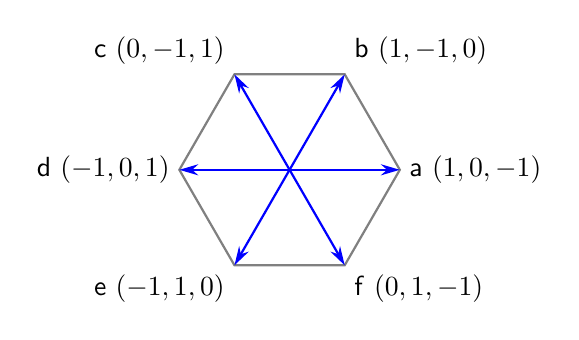
\begin{tikzpicture}[scale=1.4]
  % Hexagon
  \draw[gray, thick]
    (0:1) -- (60:1) -- (120:1) -- (180:1) -- (240:1) -- (300:1) -- cycle;

  % Red arrows (a, c, e directions)
  \draw[-{Stealth[length=2.4mm,width=1.4mm]}, blue, thick] (0,0) -- (1,0);       % a direction
  \draw[-{Stealth[length=2.4mm,width=1.4mm]}, blue, thick] (0,0) -- (0.5,0.866);       % b direction
  \draw[-{Stealth[length=2.4mm,width=1.4mm]}, blue, thick] (0,0) -- (-0.5,0.866);  % c direction
  \draw[-{Stealth[length=2.4mm,width=1.4mm]}, blue, thick] (0,0) -- (-1,0);       % d direction
  \draw[-{Stealth[length=2.4mm,width=1.4mm]}, blue, thick] (0,0) -- (-0.5,-0.866);  % e direction
  \draw[-{Stealth[length=2.4mm,width=1.4mm]}, blue, thick] (0,0) -- (0.5,-0.866);  % f direction

  % Labels
  \node[right] at (1,0) {\textsf{a} \textsf{$(1,0,-1)$}};
  \node[above right] at (0.5,0.866) {\textsf{b} \textsf{$(1,-1,0)$}};
  \node[above left] at (-0.5,0.866) {\textsf{c} \textsf{$(0,-1,1)$}};
  \node[left] at (-1,0) {\textsf{d} \textsf{$(-1,0,1)$}};
  \node[below left] at (-0.5,-0.866) {\textsf{e} \textsf{$(-1,1,0)$}};
  \node[below right] at (0.5,-0.866) {\textsf{f} \textsf{$(0,1,-1)$}};
\end{tikzpicture}
\end{center}



Perfect polyiamonds can be represented as strings over the alphabet 
$\Sigma = \{ \mathtt{a}, \mathtt{b}, \mathtt{c}, \mathtt{d}, \mathtt{e}, \mathtt{f} \}$ 
listing their side directions in decreasing length order.
Specifying the lengths is not necessary, as they are determined 
by the position in the string.
The set of all perfect polyiamonds can be viewed as a language over $\Sigma$: 

$$\mathcal{P} = \{ w \in \Sigma^* \mid w \text{ encodes a perfect polyiamond} \}.$$

To avoid symmetric cases (rotations and reflections),
we typically assume that the longest side for an encoded perfect polyiamond 
is in direction $\mathtt{a}$, and the second longest side is 
either in direction $\mathtt{b}$ or $\mathtt{c}$, so that the first 
two symbols of the string are $\mathtt{a}\mathtt{b}$ or $\mathtt{a}\mathtt{c}$.


\begin{definition}
The set $\mathcal{A} \subseteq \mathcal{P}$ of all perfect acute polyiamonds 
with internal angles $60^\circ$ or $300^\circ$.
The set $\mathcal{O} \subseteq \mathcal{P}$ of all perfect obtuse polyiamonds 
with internal angles $120^\circ$ or $240^\circ$.
\end{definition}


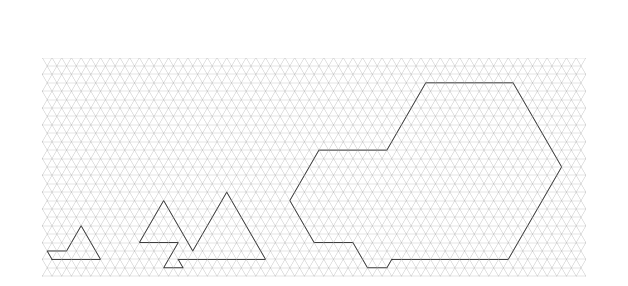
\includegraphics[width=0.8\textwidth]{polyiamond-examples.png}




\section{Results}

{\bf The necessary conditions for the existence of perfect acute polyiamonds:}

\begin{proposition}
A perfect acute n-polyiamond can only exist if
$n \equiv 3 \pmod{6}$ or $n \equiv 5 \pmod{6}$.
\end{proposition}

\textbf{Proof:}

\noindent (1) Side directions are ``\textbf{a}'', ``\textbf{c}'' or ``\textbf{e}''.
The sides $\{1, 2, \ldots, n\}$ are split into 3
disjoint subsets of equal sums.
Hence $\dfrac{n(n+1)}{2}$ is divisible by 3.

\medskip

\noindent (2) For even $n = 2k$ the sum of
internal angles is $(2k - 2) \cdot 180^\circ$.
Let $m$ of these angles be $60^\circ$. Then

\begin{align*}
(2k - 2) \cdot 180^\circ &= m \cdot 60^\circ + (2k - m) \cdot 300^\circ \\
6k - 6 &= m + (2k - m) \cdot 5 \\
4m &= 4k + 6 \\
0 &\equiv 2 \pmod{4}
\end{align*}

A contradiction. \qedsymbol





\begin{proposition}
A perfect obtuse n-polyiamond can only exist if
\[
n \equiv 0 \pmod{6}
\]
\end{proposition}

\textbf{Proof:} 
For odd $n = 2k + 1$ the sum of inner angles:

\begin{align*}
180^\circ(2k - 1) &= 120^\circ m + 240^\circ(2k - 1 - m) \\
3(2k - 1) &= 2m + 4(2k - 1 - m) \\
1 &\equiv 0 \pmod{2}
\end{align*}

Contradiction. So $n$ must be even.



\medskip

For red direction vectors $(\mathtt{a},\mathtt{c},\mathtt{e})$ we have
\[ x - y \equiv 1 \pmod{3} \]
For blue direction vectors $(\mathtt{b},\mathtt{d},\mathtt{f})$ we have
\[ x - y \equiv 2 \pmod{3} \]
In an obtuse polyiamond they alternate -- all red
vectors are even; blue vectors are odd.
Adding any side of a perfect obtuse polyiamond
increases the difference $(x - y)$ by $2 \pmod{3}$.
So the number of sides $\boldsymbol{n}$ is divisible by 3. \qedsymbol






\begin{proposition}
There is no infinite set of perfect polyiamonds that is a 
regular language over $\Sigma$. 
({\em Hint:} Apply Pumping lemma.)
\end{proposition}



\begin{proposition}
There is an infinite set of perfect polyiamonds generated by a context-free grammar; 
(Examples in \cite{RudzateApsitis2024}.)
\end{proposition}

\begin{tabular}{ |l|l| } 
\hline
Perfect polyiamonds & Acute perfect polyiamonds \\ 
$S \rightarrow \mathtt{acec}P\mathtt{db}$, & 
$S \rightarrow \mathtt{acaeae}P\mathtt{eacacac}$, \\ 
$P \rightarrow \mathtt{ecea}P\mathtt{abcb} \,\mid\, \mathtt{eceaeafabcb}.$ & 
$P \rightarrow \mathtt{aececacece}P(\mathtt{caea})^5 \,\mid\, \mathtt{cecececa}.$\\ 
\hline
\end{tabular}




\begin{proposition}
There is a {\em parallel context-free language (PCL)}\cite{Siromoney1974} 
generating an infinite two-dimensional family of perfect polyiamonds.
% express this with PCL rules: {\tt \url{https://bit.ly/3UoJnkq}}.
\end{proposition}

\begin{proposition}
For $n = 27, 35, 171, 275, 1595$, a perfect acute $n$-polyiamond with the 
maximum area among all perfect acute $n$-polyiamonds has a 
triangular shape and matches the regex 
$\mathtt{a}(\mathtt{ca})^{+}(\mathtt{ea})^{+}(\mathtt{ec})^{+}(\mathtt{ac})^{+}$. 
\end{proposition}


\begin{thebibliography}{10}

\bibitem{APSITIS1}
%(TODO) Atsauce uz rakstu, kur pirmoreiz nodefinēti perfektie polimondi.
Buliņa, E. \textit{Maģiskie polimondi un to īpašības} [{\it Magic Polyiamonds and their Properties}], Master's thesis, University of Latvia. Available at: {\tt https://dspace.lu.lv/dspace/handle/7/38915}
\bibitem{Joshi1997}
Joshi, A.K., Schabes, Y.
{\it Tree-Adjoining Grammars.}
In "Handbook of Formal Languages" (Volume 3), Springer, (1997) 69--123.
\bibitem{RudzateApsitis2024}
Rudzāte, M., Apsītis, K.
{\it Notes for the 'Families of Perfect Polyiamonds'.} 
Available at: {\tt https://bit.ly/49mqmmL}
\bibitem{Siromoney1974}
Siromoney, R., Krithivasan, K.
{\it Parallel Context-Free Languages.}
Information and Control. {\bf 24} (1974) 155--162. 

\end{thebibliography}




\end{document}

